\documentclass[a4paper,openright,12pt]{report}
\usepackage[latin1]{inputenc}
\usepackage[spanish]{babel}
\usepackage{amsmath}
\usepackage{amsfonts}
\usepackage{amssymb}
\usepackage{graphicx}
\usepackage{multicol}
\usepackage{changepage}

\usepackage{cite}
\usepackage{url}


\usepackage[left=4cm,right=3cm,top=4cm,bottom=3cm]{geometry}
\author{Elisban Vilca Mamani}
\title{Mi portada}

\begin{document}
%------------encabezado
	\pagestyle{plain}{
		\pagestyle{empty}
		\changepage{3cm}{1cm}{-0.5cm}{-0.5cm}{}{-2cm}{}{}{}
		{\small
		 
		}
%-----------datos de la caratula
			\begin{center}
			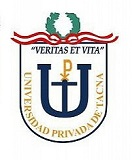
\includegraphics[scale=1]{upt.jpg}
			
				\par\vspace{2cm}%-------espacio dejado antes del encabezado
			{
				\huge\textbf{
						UNIVERSIDAD PRIVADA DE TACNA \\*[0.20cm] Escuela Profesional de Ingenieria de Sistemas e Informatica}
			}
			\par\vspace{3cm}
			{	
				\large\textbf{Curso: Base de datos II \\ Asesor: Patrick Cuadros Quiroga \\ Alumno: Elisban Vilca Mamani \\ Trabajo: Nikola Tesla}
			}
			\end{center}

		}	
%--------indice




\tableofcontents
\begin{large}
\chapter{Biografia}
\begin{flushleft}
Nikola Tesla era hijo de padres serbios en el pueblo de Smiljan, en el Imperio austrohungaro, cerca de la ciudad de Gospić, perteneciente al territorio de la actual Croacia. Su certificado de bautismo afirma que nació el 28 de junio de 1856 del calendario juliano, correspondiente al 10 de julio del calendario gregoriano en uso actualmente. Su padre fue Milutin Tesla, un sacerdote de la iglesia ortodoxa serbia en la jurisdicción de Sremski Karlovci, y su madre Đuka Mandici, una ama de casa de ascendencia serbia,​ y quien dedicaba parte de su tiempo como científica autodidacta al desarrollo de pequeños aparatos caseros.

Se cree que su origen paterno proviene de alguno de los clanes serbios del valle del río Tara, o bien del noble herzegovino Pavle Orlović.​ Su madre, Đuka, provenía de una familia ortodoxa domiciliada en Lika y Banija, pero con profundos orígenes en Kosovo.​ Era competente fabricando herramientas artesanales caseras y había aprendido de memoria numerosos poemas épicos serbios, pero nunca aprendió a leer.....\\
\end{flushleft}


\chapter{Premios}\label{cap.nudo}
\begin{flushleft}
A pesar de que el premio Nobel de física fue otorgado a Marconi por la invención de la radio en 1909, la prensa publicó que Edison y Tesla compartirían el premio Nobel en 1915. Edison trató de minimizar los logros de Tesla y se negó a recibir el premio en caso de que fuera compartido. Algunas fuentes afirmaron que debido a la envidia de Edison ninguno lo ganó, a pesar de sus grandes contribuciones a la ciencia.​ Antes, se decía que Tesla podía ser nominado para el premio Nobel de 1912. La nominación se debía posiblemente a sus circuitos sintonizados usando transformadores resonantes de alta tensión y alta frecuencia. La investigación histórica posterior demostró que en esa época el nombre de Tesla no fue considerado para el premio Nobel, aunque alguna prensa sí que habló de ello.

Tesla solo fue premiado con la medalla Edison, la máxima distinción otorgada por la IEEE.
La unidad utilizada en el Sistema Internacional para medir la inducción magnética se llama tesla en su memoria.\\

\vspace*{0.6in}

\begin{center}
{\Large 1 T = 1 Wb·m−2 = 1 kg·s−2·A−1 = 1 kg·C-1·s-1}
\end{center}
\end{flushleft}

\chapter{Fotos}\label{cap.desenlace}
\begin{center}
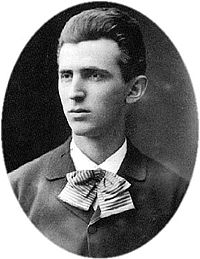
\includegraphics[width=4cm]{Tesla.jpg}
\end{center}

\end{large}
%FIN INDICE



\end{document}


